\chapter{Requirements}
\section{Allgemeine Beschreibung}
\subsection{Produktperspektive}
Mit Internet of Things sind eine Vielzahl neuartige Devices entstanden. Während in herkömmlichen Netzwerken hauptsächlich Personal Computer, Notebooks, Server usw. verwaltet werden mussten, so bringen IoT Devices den IT-Abteilungen neue Herausforderungen. Zum einen dürfte die Anzahl Geräte gegenüber herkömmlichen Computer deutlich ansteigen, zum anderen sind IoT Devices in Sachen Funktionalität und Rechenleistung, sowie auch der Netzwerkbandbreite deutlich beschränkt. 

Mit <insert Application Name here> soll eine Management Applikation bereitgestellt werden, um eine Vielzahl unterschiedlicher IoT Devices administrieren zu können. 
\subsection{Produkfunktionen}
<insert Application Name here> soll den Benutzern erlauben, IoT Geräte zu verwalten. Die Aufgaben reichen vom Erfassen und Discovery von Devices über die Konfigurationsverwaltung und Softwareverteilung bis zu Backup und Restore. Ausserdem sollen Management-relevante Kommandos auf Devices ausgeführt- und Security Aspekte beachtet werden. Die Details zu den Produktfunktionen sind den Use Cases zu entnehmen.

\subsection{Benutzer Charakteristik}
Zielpersonen der Applikation sind Betreiber von IoT Devices. Dies können im Enterprise Umfeld IT-Mitarbeiter in operationeller Funktion-, oder auch Softwareentwickler für IoT Applikationen sein. Heimanwender können bei entsprechenden Kenntnissen ebenfalls zur Zielgruppe gehören. Es werden solide Grundkenntnisse in TCP/IP Netzwerken sowie Verständnis der verwendeten IoT Architekturen und Devices vorausgesetzt. 
\subsection{Einschränkungen}
Evtl. Browser Einschränkungen und bestimmte Use Cases, müsste nach Prototyp nochmals definiert werden
\section{Use Cases}
\subsection{Use Cases Diagramm}
\begin{figure}[H]
\centering
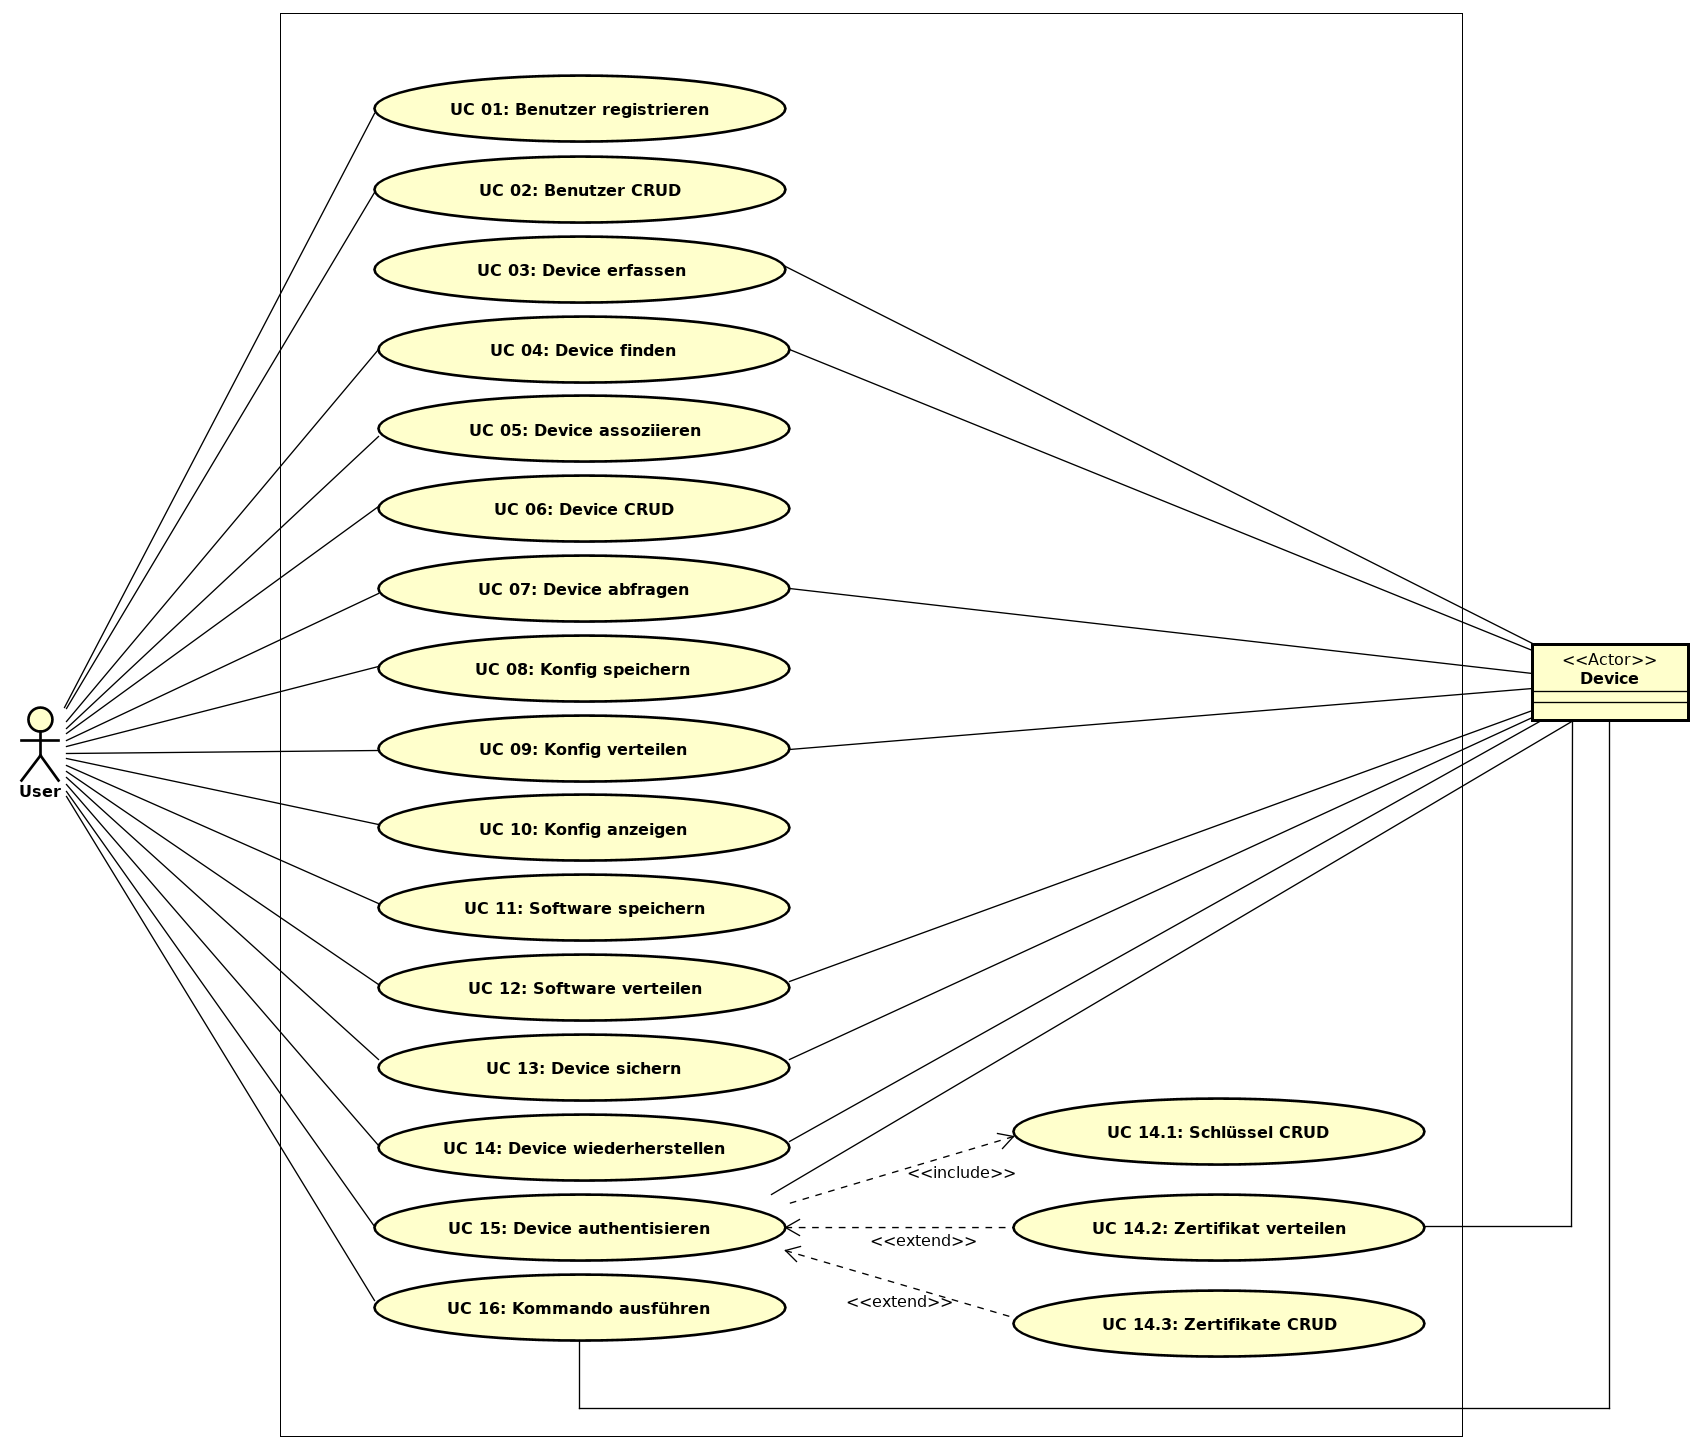
\includegraphics[scale=0.425]{images/use_case_diagram.png}\caption{Use Case Diagramm}
\end{figure}
\subsection{Aktoren}
Der Benutzer der Applikation ist in diesem System der einzige primäre Aktor.
\newpage
\subsection{Beschreibungen (Casual)}
\subsubsection{Benutzer CRUD}
\mbox{}
\begin{longtable}{| p{4cm} | p{11.7cm} |}
 \hline
 \textbf{ID} & 01\\ \hline 
 \textbf{Name} & Benutzer CRUD\\ \hline 
 \textbf{Beschreibung} & Benutzerverwaltung der Applikation\\ \hline 
 \textbf{Preconditions} & 
   \tabitem Applikation gestartet \newline
   \tabitem Benutzer ist registriert \newline
   \tabitem Benutzer ist eingeloggt 
  \\ \hline 
 \textbf{Postconditions} & 
  \tabitem Änderungen gespeichert
 \\ \hline
 \textbf{Main Success Scenario} &
 \textbf{Create:}\newline
  1. UC 01: Benutzer registrieren \newline
 \textbf{Read:}\newline
  1. Benutzer lässt Userdaten anzeigen \newline
 \textbf{Update:}\newline
  1. Benutzer lässt Userdaten anzeigen \newline
  2. Benutzer verändert Attribute\newline
  3. Benutzer speichert Änderungen\newline
 \textbf{Delete:}\newline
  1. Benutzer wird gelöscht \\ 
 \hline 
 \textbf{Extensions} & -\\ \hline 
 \end{longtable}

\subsubsection{Device erfassen}
\mbox{}
\begin{longtable}{| p{4cm} | p{11.7cm} |}
 \hline
 \textbf{ID} & 02\\ \hline 
 \textbf{Name} & Device erfassen \\ \hline 
 \textbf{Beschreibung} & Der Benutzer möchte ein Device manuell hinzufügen. Der Endpunkt ist dem Benutzer bekannt. 
 \\ \hline 
 \textbf{Preconditions} & 
   \tabitem Applikation gestartet \newline
   \tabitem Benutzer eingeloggt \newline
   \tabitem Device Endpunkt ist dem Benutzer bekannt
  \\ \hline 
 \textbf{Postconditions} & 
  \tabitem Falls ein Gerät gefunden wird, wird es angezeigt 
  \\ \hline 
 \textbf{Main Success Scenario} & 
  1. Benutzer öffnet Device Erfassung \newline
  2. Benutzer gibt Device Endpunkt ein \newline
  3. Benutzer startet Suchvorgang \newline
  4. Anfrage wird an Device gesendet \newline
  5. Antwort vom Device wird angezeigt
 \\ \hline 
 \textbf{Extensions} & 
  5.a Timeout Fehlermeldung wird dem Benutzer angezeigt 
  \\ \hline 
\end{longtable}
\newpage
\subsubsection{Device finden}
\mbox{}
\begin{longtable}{| p{4cm} | p{11.7cm} |}
 \hline
 \textbf{ID} & 03\\ \hline 
 \textbf{Name} & Device finden\\ \hline 
 \textbf{Beschreibung} & Der Benutzer möchte ein- oder meherere Devices finden. Endpunkt des Devices ist dem Benutzer unbekannt. Gefundene Devices sollen dem Benutzer aufgelistet werden. \\ \hline 
 \textbf{Preconditions} &  
  \tabitem Applikation gestartet \newline
  \tabitem Benutzer eingeloggt
 \\ \hline 
 \textbf{Postconditions} & 
  \tabitem Gefundene Devices werden dem Benutzer angezeigt 
 \\ \hline 
 \textbf{Main Success Scenario} & 
  1. Benutzer öffnet Device Discovery \newline
  2. System listet eingegangene Anfragen von Devices auf \newline
  3. Benutzer wählt gewünschte Devices aus  
 \\ \hline 
 \textbf{Extensions} &  
  2.a System zeigt Fehlermeldung an
 \\ \hline 
 \end{longtable}
 
\subsubsection{Device assoziieren}
\mbox{}
\begin{longtable}{| p{4cm} | p{11.7cm} |}
 \hline
 \textbf{ID} & 04\\ \hline 
 \textbf{Name} & Device assoziieren \\ \hline 
 \textbf{Beschreibung} & Der Benutzer möchte ein Device verwalten. Dazu muss er das gefundene Device in das System adoptieren.   \\ \hline 
 \textbf{Preconditions} & 
  \tabitem Applikation gestartet \newline
  \tabitem Benutzer eingeloggt \newline
  \tabitem Mindestens 1 Device gefunden 
 \\ \hline 
 \textbf{Postconditions} & 
  \tabitem Assoziation zu gefundemen Device erstellt 
 \\ \hline 
 \textbf{Main Success Scenario} &
  1. Benutzer erstellt Assoziation von gefundenen Devices (UC 02 / UC 03)
 \\ \hline 
 \textbf{Extensions} & -\\ \hline 
 \end{longtable}
 
\subsubsection{Device CRUD}
\mbox{}
\begin{longtable}{| p{4cm} | p{11.7cm} |}
 \hline
 \textbf{ID} & 05\\ \hline 
 \textbf{Name} & Device CRUD\\ \hline 
 \textbf{Beschreibung} & Deviceverwaltung der Applikation\\ \hline 
 \textbf{Preconditions} & 
  \tabitem Applikation gestartet \newline
  \tabitem Benutzer eingeloggt
 \\ \hline 
 \textbf{Postconditions} & 
  \tabitem Änderungen gespeichert 
 \\ \hline 
 \textbf{Main Success Scenario} &
 \textbf{Create:}\newline
  1. UC 04: Device assoziieren \newline
 \textbf{Read:}\newline
  1. Attribute eines Devices anzeigen \newline
 \textbf{Update:}\newline
  1. Benutzer lässt Device Attribute anzeigen \newline
  2. Benutzer verändert Attribute\newline
  3. Benutzer speichert Änderungen\newline
 \textbf{Delete:}\newline
  1. Device Assoziation wird gelöscht 
  \\ \hline 
 \textbf{Extensions} & -\\ \hline 
 \end{longtable}
 
\subsubsection{Device abfragen}
\mbox{}
\begin{longtable}{| p{4cm} | p{11.7cm} |}
 \hline
 \textbf{ID} & 06\\ \hline 
 \textbf{Name} & Device abfragen\\ \hline 
 \textbf{Beschreibung} & Gewünschte Parameter und Attribute werden vom Device abgefragt\\ \hline 
 \textbf{Preconditions} &  
  \tabitem Applikation gestartet \newline
  \tabitem Benutzer eingeloggt 
 \\ \hline 
 \textbf{Postconditions} & 
  \tabitem Antwort vom Device oder Fehlermeldung wird angezeigt 
 \\ \hline 
 \textbf{Main Success Scenario} & 
  1. Benutzer wählt Device aus \newline
  2. Benutzer startet Abfrage \newline
  3. System sendet Anfrage an Device \newline
  4. System speichert Antwort (UC 05: Device CRUD)
 \\ \hline 
 \textbf{Extensions} & 
  1.a Benutzer wählt mehrere Devices aus \newline
  3.a System sendet Anfragen an mehrere Devices
 \\ \hline 
 \end{longtable}
 
\subsubsection{Konfiguration speichern}
\mbox{}
\begin{longtable}{| p{4cm} | p{11.7cm} |}
 \hline
 \textbf{ID} & 07\\ \hline 
 \textbf{Name} & Konfiguration speichern\\ \hline 
 \textbf{Beschreibung} &  Konfigurationen von beliebigen Devices können im System gespeichert werden\\ \hline 
 \textbf{Preconditions} &
  \tabitem Applikation gestartet \newline
  \tabitem Benutzer eingeloggt \newline
  \tabitem Konfigurationsfile für Benutzer zugänglich   
 \\ \hline 
 \textbf{Postconditions} & 
  \tabitem Konfigurationsfile im System gespeichert
 \\ \hline 
 \textbf{Main Success Scenario} & 
  1. Benutzer lädt Konfigurationsfile in System 
 \\ \hline 
 \textbf{Extensions} & -\\ \hline 
 \end{longtable}
 
\subsubsection{Konfiguration verteilen}
\mbox{}
\begin{longtable}{| p{4cm} | p{11.7cm} |}
 \hline
 \textbf{ID} & 08\\ \hline 
 \textbf{Name} & Konfiguration verteilen\\ \hline 
 \textbf{Beschreibung} & Konfigurationen können an Devices versendet werden.\\ \hline 
 \textbf{Preconditions} &  
  \tabitem Applikation gestartet \newline
  \tabitem Benutzer eingeloggt
  \tabitem Konfiguration im System vorhanden 
 \\ \hline 
 \textbf{Postconditions} & Konfiguration an Device geschickt\\ \hline 
 \textbf{Main Success Scenario} & 
  1. Benutzer wählt Device aus \newline
  2. Benutzer wählt Konfiguration aus \newline
  3. Benutzer versendet Konfiguration \newline
  4. System zeigt Antwort des Devices an 
 \\ \hline 
 \textbf{Extensions} &
  1.a Benutzer wählt mehrere Device aus
  4.a System zeigt Antworten mehrerer Devices an
 \\ \hline 
 \end{longtable}
 
\subsubsection{Konfiguration anzeigen}
\mbox{}
\begin{longtable}{| p{4cm} | p{11.7cm} |}
 \hline
 \textbf{ID} & 09\\ \hline 
 \textbf{Name} & Konfiguration anzeigen\\ \hline 
 \textbf{Beschreibung} & Konfigurationsdetails im System können angesehen werden\\ \hline 
 \textbf{Preconditions} &  
  \tabitem Applikation gestartet \newline
  \tabitem Benutzer eingeloggt \newline
  \tabitem Konfiguration im System vorhanden 
 \\ \hline 
 \textbf{Postconditions} & 
  \tabitem Konfigurationsdetails angezeigt 
 \\ \hline 
 \textbf{Main Success Scenario} &  
  1. Benutzer wählt Konfiguration aus \newline
  2. System zeigt Konfiguration an 
 \\ \hline 
 \textbf{Extensions} & -\\ \hline 
 \end{longtable}
 
\subsubsection{Software speichern}
\mbox{}
\begin{longtable}{| p{4cm} | p{11.7cm} |}
 \hline
 \textbf{ID} & 10\\ \hline 
 \textbf{Name} & Software speichern\\ \hline 
 \textbf{Beschreibung} & Spezifische Software oder Firmware für Devices können im System gespeichert werden.\\ \hline 
 \textbf{Preconditions} &
  \tabitem Applikation gestartet \newline
  \tabitem Benutzer eingeloggt \newline
  \tabitem Softwarefile für Benutzer zugänglich 
 \\ \hline 
 \textbf{Postconditions} & 
  \tabitem Softwarefile im System gespeichert
 \\ \hline 
 \textbf{Main Success Scenario} &
  1. Benutzer lädt Softwarefile in System
 \\ \hline 
 \textbf{Extensions} & -\\ \hline 
 \end{longtable}
 
\subsubsection{Software verteilen}
\mbox{}
\begin{longtable}{| p{4cm} | p{11.7cm} |}
 \hline
 \textbf{ID} & 11\\ \hline 
 \textbf{Name} & Software verteilen\\ \hline 
 \textbf{Beschreibung} & • \\ \hline 
 \textbf{Preconditions} & • \\ \hline 
 \textbf{Postconditions} & • \\ \hline 
 \textbf{Main Success Scenario} & • \\ \hline 
 \textbf{Extensions} & • \\ \hline 
 \end{longtable}
 
\subsubsection{Device sichern}
\mbox{}
\begin{longtable}{| p{4cm} | p{11.7cm} |}
 \hline
 \textbf{ID} & 12\\ \hline 
 \textbf{Name} & Device sichern\\ \hline 
 \textbf{Beschreibung} & • \\ \hline 
 \textbf{Preconditions} & • \\ \hline 
 \textbf{Postconditions} & • \\ \hline 
 \textbf{Main Success Scenario} & • \\ \hline 
 \textbf{Extensions} & • \\ \hline 
 \end{longtable}
 
\subsubsection{Device wiederherstellen}
\mbox{}
\begin{longtable}{| p{4cm} | p{11.7cm} |}
 \hline
 \textbf{ID} & 13\\ \hline 
 \textbf{Name} & Device wiederherstellen\\ \hline 
 \textbf{Beschreibung} & • \\ \hline 
 \textbf{Preconditions} & • \\ \hline 
 \textbf{Postconditions} & • \\ \hline 
 \textbf{Main Success Scenario} & • \\ \hline 
 \textbf{Extensions} & • \\ \hline 
 \end{longtable}
 
\subsubsection{Device authentisieren}
\mbox{}
\begin{longtable}{| p{4cm} | p{11.7cm} |}
 \hline
 \textbf{ID} & 14\\ \hline 
 \textbf{Name} & Device authentisieren\\ \hline 
 \textbf{Beschreibung} & • \\ \hline 
 \textbf{Preconditions} & • \\ \hline 
 \textbf{Postconditions} & • \\ \hline 
 \textbf{Main Success Scenario} & • \\ \hline 
 \textbf{Extensions} & • \\ \hline 
 \end{longtable}
 
\subsubsection{Schlüssel verwalten}
\mbox{}
\begin{longtable}{| p{4cm} | p{11.7cm} |}
 \hline
 \textbf{ID} & 14.1\\ \hline 
 \textbf{Name} & Schlüssel verwalten\\ \hline 
 \textbf{Beschreibung} & • \\ \hline 
 \textbf{Preconditions} & • \\ \hline 
 \textbf{Postconditions} & • \\ \hline 
 \textbf{Main Success Scenario} & • \\ \hline 
 \textbf{Extensions} & • \\ \hline 
 \end{longtable}
 
\subsubsection{Zertifikate verteilen}
\mbox{}
\begin{longtable}{| p{4cm} | p{11.7cm} |}
 \hline
 \textbf{ID} & 14.2\\ \hline 
 \textbf{Name} & Zertifikate verteilen\\ \hline 
 \textbf{Beschreibung} & • \\ \hline 
 \textbf{Preconditions} & • \\ \hline 
 \textbf{Postconditions} & • \\ \hline 
 \textbf{Main Success Scenario} & • \\ \hline 
 \textbf{Extensions} & • \\ \hline 
 \end{longtable}
 
\subsubsection{Zertifikate CRUD}
\mbox{}
\begin{longtable}{| p{4cm} | p{11.7cm} |}
 \hline
 \textbf{ID} & 14.3\\ \hline 
 \textbf{Name} & Zertifikate CRUD\\ \hline 
 \textbf{Beschreibung} & • \\ \hline 
 \textbf{Preconditions} & • \\ \hline 
 \textbf{Postconditions} & • \\ \hline 
 \textbf{Main Success Scenario} & • \\ \hline 
 \textbf{Extensions} & • \\ \hline 
 \end{longtable} 
 
\subsubsection{Device Kommandos ausführen}
\mbox{}
\begin{longtable}{| p{4cm} | p{11.7cm} |}
 \hline
 \textbf{ID} & 15\\ \hline 
 \textbf{Name} & Device Kommandos ausführen\\ \hline 
 \textbf{Beschreibung} & • \\ \hline 
 \textbf{Preconditions} & • \\ \hline 
 \textbf{Postconditions} & • \\ \hline 
 \textbf{Main Success Scenario} & • \\ \hline 
 \textbf{Extensions} & • \\ \hline 
\end{longtable}


 
 

\section{Nichtfunktionale Anforderungen}
In diesem Kapitel behandeln wir die nichtfunktionalen Anforderungen an das Projekt. Wir behandeln Aspekte und Anforderungen aus den Bereichen Qualität, Schnittstellen und Randbedingungen.
\subsection{Qualität}
Bei der Softwarequalität stützen wir uns auf die ISO/IEC 9126 Norm. Es werden die Merkmale Funktionalität, Zuverlässigkeit, Benutzbarkeit, Effizienz, Wartbarkeit und Übertragbarkeit aufgeführt.
\subsubsection{Funktionalität}
Netzwerkdevices können von vielen unterschiedlichen Herstellern kommen. Diese Hersteller verwenden unterschiedliche Syntax und Ausgabeformate. Um die Funktionalität best möglich sicherzustellen, wird die Herstellerunterstützung vorerst stark eingeschränkt. Vorgesehen sind vorerst Cisco Netzwerkdevices und Linux Hosts.
\subsubsection{Zuverlässigkeit}
Tests sind wichtig und nützlich, jedoch nicht Business kritisch bei einem möglichen Ausfall. Es muss vor allem darauf geachtet werden, dass bei ssh Verbindungen ein sauberes Exception Handling implementiert wird, falls beim Verbindungsaufbau oder bei abgesetzten Kommandos etwas schief geht. Es müssen für gewisse Tests auch Timeouts eingeplant werden, damit das Programm nicht unendlich lange blockieren kann.
\subsubsection{Benutzbarkeit}
Wir möchten ein schmales User Interface auf Konsolen Ebene bieten. Der Anwender muss über Kenntnisse auf der Linux bash verfügen. Mittels eingebauter Hilfe soll es versierten Benutzern möglich sein, die Software zu verwenden.
\subsubsection{Effizienz}
Die Effizienz ist sehr stark von den getesteten Devices und den abgesetzten Kommandos abhängig. 
\subsubsection{Wartbarkeit}
Eigene Test Cases sollen mit den notwendigen Kenntnissen selbst ergänzt werden können. Command-Mapping und Outputs müssen bekannt sein, dann ist eine Erweiterung des Funktionsumfangs der Test Cases denkbar.
\subsubsection{Übertragbarkeit}
Die Übertragbarkeit auf andere Plattformen oder Hersteller ist schwierig und vorerst nicht vorgesehen.

\subsection{Schnittstellen}
\subsubsection{Benutzerschnittstellen}
Die Steuerung des Programms ist mittels Tastatur über die Linux bash vorgesehen.

\subsubsection{Netzwerkschnittstellen}
Im Programm können alle Devices verwendet werden, welche über ein lokales Netzwerkinterface erreichbar sind.

\subsection{Sicherheit}
Um auf Devices verbinden zu können, muss man sich auf diesen authentifizieren. Administrator Zugänge müssen deshalb best möglichst geschützt sein. Die Übertragung muss verschlüsselt sein (ssh) und die Passwörter dürfen, wenn überhaupt, nur mittels sicherem Hashverfahren abgelegt werden.